% ----------------------------------------------------------------------
%  Před psaním se důkladně seznamte s Pravidly pro vypracování protokolu!
% ----------------------------------------------------------------------

% ----------------------------------------------------------------------
%  Pracovní úkoly - opište přímo ze zadání
% ----------------------------------------------------------------------
\section{Pracovní úkoly}

\begin{enumerate}
\item Nastavte zesílení proporcionálního členu na 1 ($R_P=R'_P=10 \unit{k\Omega}$). Dále vyřaďte integrační ($R_I=\infty$ a $C_I=0 \unit{nF}$) a derivační člen ($C_D=\infty$ a $R_D=0 \unit{\Omega}$).
\item Změřte statickou charakteristiku soustavy v otevřené smyčce. Hodnoty vyneste do grafu (závislost otáček za minutu na řídící veličině). Rozsah řídící veličiny bude od -1.6 V do 1.6 V.
\begin{enumerate}
	\item Je tato charakteristika lineární nebo nelineární, případně v jakém rozsahu je lineární?
	\item Vyjádřete funkční závislost statické charakteristiky lineární funkcí.
\end{enumerate}
\item Změřte přechodovou charakteristiku soustavy v otevřené smyčce. Hodnoty vyneste do grafu (závislost napětí z tachogenerátoru na čase). Řídící veličina se skokově změní z 0.6 V na 1.6 V.
\item Dle změřené přechodové charakteristiky identifikujte strukturu a řád modelu soustavy.
\begin{enumerate}
	\item Jaká je obecná přenosová funkce tohoto modelu?
	\item Popište parametry modelu.
	\item Metodou experimentální identifikace odhadněte parametry modelu.
	\item Ověřte průběh přechodové charakteristiky modelu s naměřenými daty.
\end{enumerate}
\item Změřte amplitudovou a fázovou frekvenční charakteristiku soustavy v otevřené smyčce. Hodnoty vyneste do grafu (závislost amplitudy [dB] / fáze [stupně] na frekvenci [log f]). Frekvenční rozsah bude od 0.1 Hz do 5 Hz.
\begin{enumerate}
	\item Jaká je frekvence zlomu?
	\item Jaká je šířka pásma soustavy?
\end{enumerate}
\item Změřte přechodovou charakteristiku soustavy v uzavřené smyčce pouze s P regulátorem se zesílením 1. Hodnoty vyneste do grafu (závislost napětí z tachogenerátoru na čase). Porovnejte přechodové charakteristiky a časové konstanty se soustavou v otevřené smyčce. Jaká je trvalá regulační odchylka?
\item Změřte amplitudovou frekvenční charakteristiku soustavy v uzavřené smyčce. Hodnoty vyneste do grafu (závislost amplitudy [dB] na frekvenci [log f]). Frekvenční rozsah bude od 0.1 Hz do 5 Hz. Jaká je frekvence zlomu? Porovnejte amplitudovou frekvenční charakteristiku se soustavou v otevřené smyčce.
\item Metodou pokus-omyl zjistěte parametry regulátoru, aby trvalá regulační odchylka byla menší než 0.3 V (cca. 300 ot./min) a časová konstanta soustavy byla menší než 20 ms.
\end{enumerate}

% ----------------------------------------------------------------------
%  Použité pomůcky
% ----------------------------------------------------------------------


\section{Sestavení experimentu}

\begin{figure}[!hbt] %bez této hranaté závorky se obrázek umístí na vrchol stránky
	\centering
	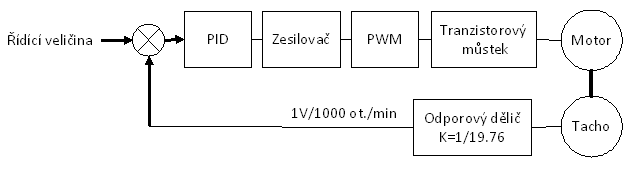
\includegraphics[]{img/schema_regulovane_soustavy.png} %nejdůležitější řádek - obsahuje cestu k obrázku a také jeho relativní šířku k šířce textu
	%všiměte si, že je možné vložit obrázek vnořený ve složce img - tam poté můžete ukládat další obrázky 
	\caption{Schéma regulované soustavy.} %popisek obrázku, který se zobrazí pod obrázkem
	\label{fig:schema_reg} %interní popis obrázku, který použijete k odkazování se
\end{figure}	

\begin{figure}[!hbt] %bez této hranaté závorky se obrázek umístí na vrchol stránky
	\centering
	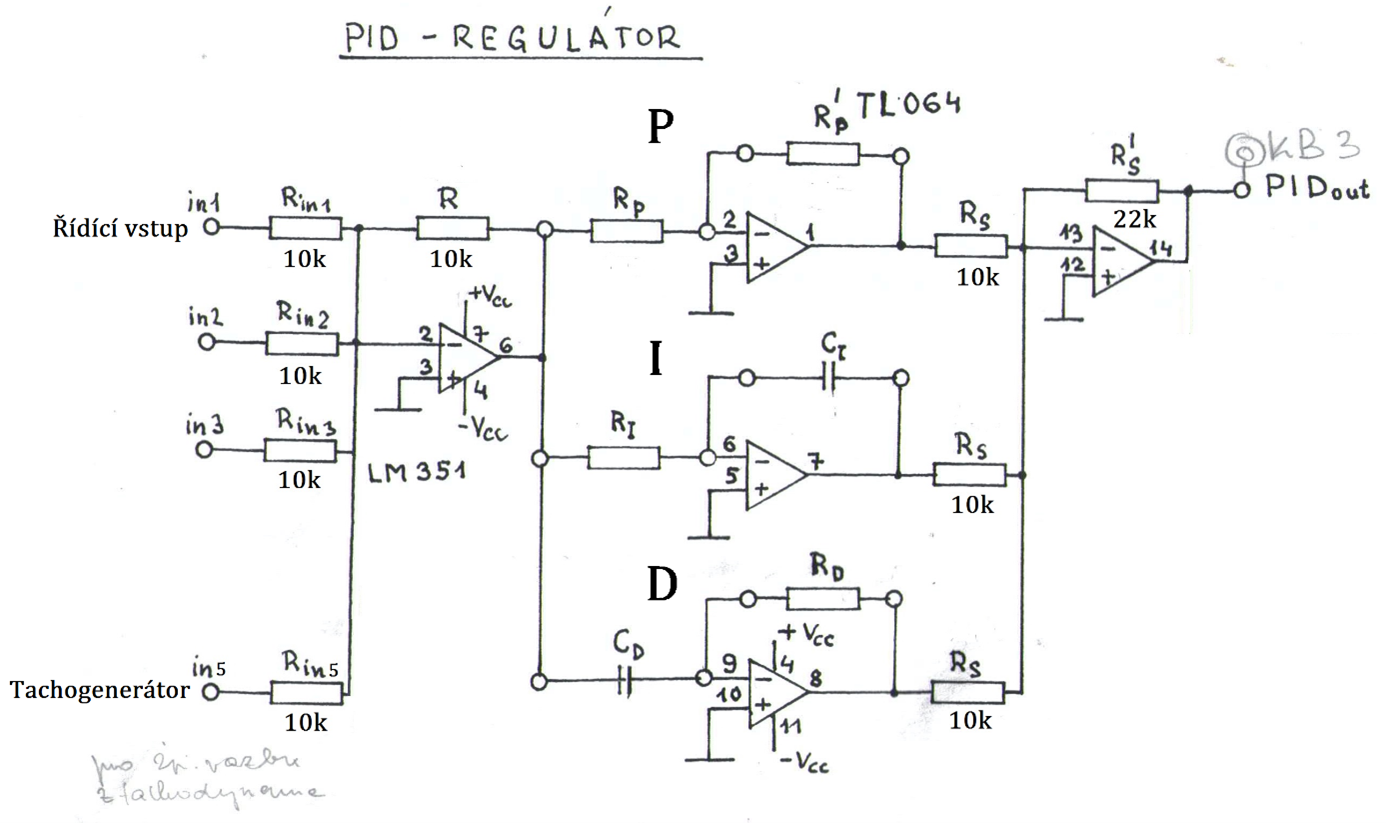
\includegraphics[]{img/schema_PID_regulatoru.png} %nejdůležitější řádek - obsahuje cestu k obrázku a také jeho relativní šířku k šířce textu
	%všiměte si, že je možné vložit obrázek vnořený ve složce img - tam poté můžete ukládat další obrázky 
	\caption{Schéma PID regulátoru.} %popisek obrázku, který se zobrazí pod obrázkem
	\label{fig:schema_PID} %interní popis obrázku, který použijete k odkazování se
\end{figure}		
		
Na obrázku Obr.\ref{fig:schema_reg} je vyobrazeno schéma regulované soustavy, na obrázku Obr.\ref{fig:schema_PID} pak schéma PID regulátoru.

% ----------------------------------------------------------------------
%  Teoretický úvod - vlastními slovy stručne popište fyzikální podstatu měření a uveďte základní vztahy použité ve vypracování
% ----------------------------------------------------------------------
%\section{Teoretický úvod}	

% ----------------------------------------------------------------------
%  Postup měření - vlastními slovy popište postup měření tak, aby bylo vaše měření reprodukovatelné 
% ----------------------------------------------------------------------
%\section{Postup měření}
			
% ----------------------------------------------------------------------
%  Naměřené hodnoty a samotné vypracování úkolu
% ----------------------------------------------------------------------				
\section{Vypracování}
	\subsection{Statická charakteristika v otevřené smyčce}
		V grafu na Obr.~\ref{fig:staticka} jsou vyneseny naměřené hodnoty statické charakteristiky soustavy v otevřené smyčce. 
		V celém rozsahu (-1.6 V - 1.6 V) statická charakteristika lineární není, avšak mezi -0.8V až -0.6V a poté 0.6V až 0.8 V ji za lineární považovat lze.
		Pro kladnou větev je funkční závislost statické charakteristiky dána předpisem $$y=(-11.9\pm 0.9)x+(-6.6\pm 0.7)$$ a pro zápornou větev pak $$y=(-10.9\pm 0.9)x+(6\pm 0.6),$$ 
		kde $y$ je výstupní veličina v mV a $x$ je vstupní veličina ve V. 
		\begin{figure}[!hbt] %bez této hranaté závorky se obrázek umístí na vrchol stránky
			\centering
			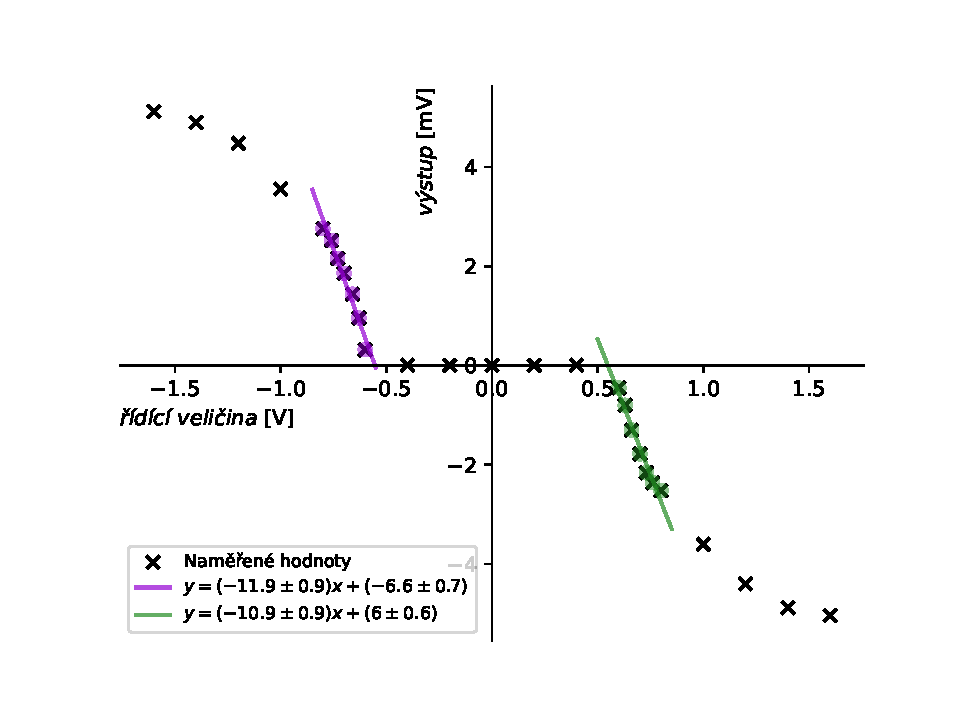
\includegraphics[]{img/graf_staticka.pdf} %nejdůležitější řádek - obsahuje cestu k obrázku a také jeho relativní šířku k šířce textu
			%všiměte si, že je možné vložit obrázek vnořený ve složce img - tam poté můžete ukládat další obrázky 
			\caption{Statická charakteristika soustavy v otevřené smyčce pro rozsah vstupní veličiny -1.6 V až 1.6 V. 
			Lineární část kladné větve (fialově) je proložena lineárním fitem $y=(-11.9\pm 0.9)x+(-6.6\pm 0.7)$, 
			lineární část záporné větve (zeleně) je fitována lineární funkcí $y=(-10.9\pm 0.9)x+(6\pm 0.6)$, 
			kde $y$ je výstupní veličina v mV a $x$ je vstupní veličina ve V.} %popisek obrázku, který se zobrazí pod obrázkem
			\label{fig:staticka} %interní popis obrázku, který použijete k odkazování se
		\end{figure}


	\subsection{Přechodová charakteristika v otevřené smyčce}
		V grafu na Obr.~\ref{fig:prechodova} je vyobrazena přechodová charakteristika soustavy v otevřené smyčce (závislost napětí z tachogenerátoru na čase) 
		pro skokovou změnu řídící veličiny z 0.6 V na 1.6 V. Fialové body jsou hodnoty přechodové charakteristiky modelu získaného odhadem parametrů a zelené body jsou naměřená data.
		Dle tvaru přechodové charakteristiky lze usoudit, že se jedná o proporcionální systém 1. řádu, který je obecně popsán přenosovou funkcí
		\begin{equation}
			\frac{k}{T\cdot s + 1},
		\end{equation}
		kde $k$ je zesílení a $T$ je časová konstanta. Tyto parametry pro měřenou soustavu jsou přibližně $k=5$ a $T=150\unit{ms}$

		\begin{figure}[!hbt] %bez této hranaté závorky se obrázek umístí na vrchol stránky
			\centering
			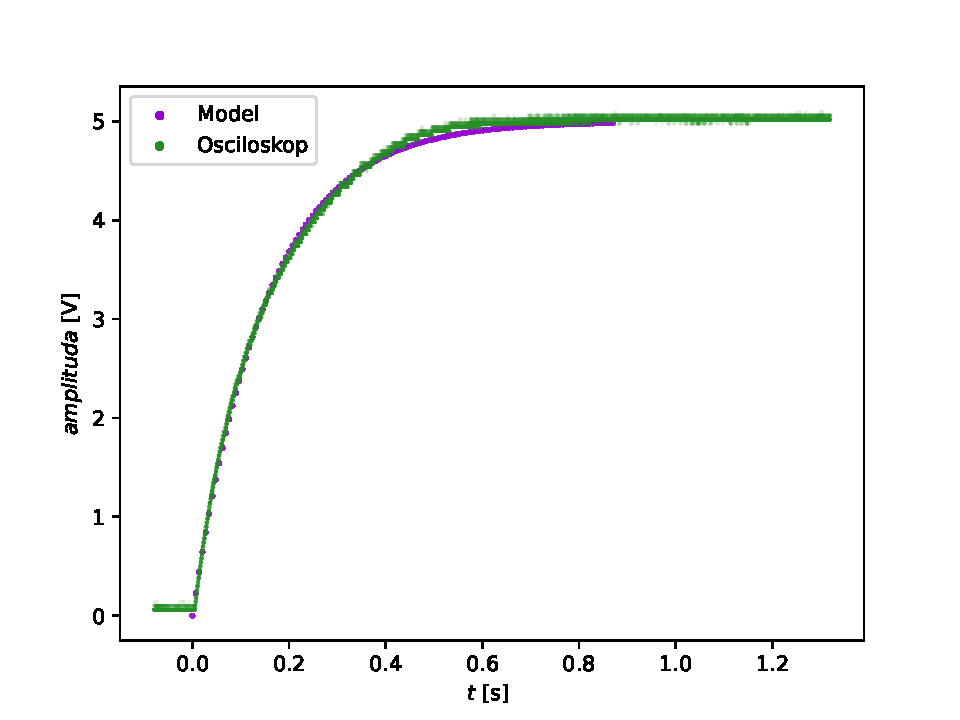
\includegraphics[]{img/graf_prechodova.pdf} %nejdůležitější řádek - obsahuje cestu k obrázku a také jeho relativní šířku k šířce textu
			%všiměte si, že je možné vložit obrázek vnořený ve složce img - tam poté můžete ukládat další obrázky 
			\caption{Přechodová charakteristika soustavy v otevřené smyčce (závislost napětí z tachogenerátoru na čase) 
			pro skokovou změnu řídící veličiny z 0.6 V na 1.6 V. 
			Fialové body jsou hodnoty přechodové charakteristiky modelu získaného odhadem parametrů a zelené body jsou naměřená data.} %popisek obrázku, který se zobrazí pod obrázkem
			\label{fig:prechodova} %interní popis obrázku, který použijete k odkazování se
		\end{figure}

	\subsection{Amplitudová a fázová frekvenční charakteristika v otevřené smyčce}

		\begin{figure}[!hbt] %bez této hranaté závorky se obrázek umístí na vrchol stránky
			\centering
			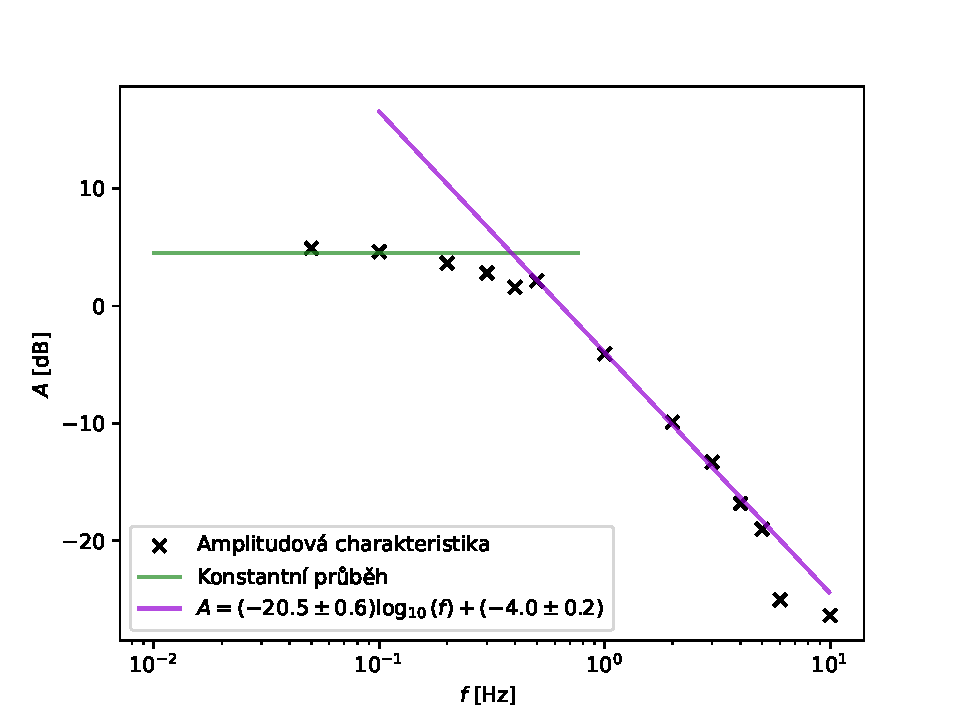
\includegraphics[]{img/graf_amplitudova_otevrena.pdf} %nejdůležitější řádek - obsahuje cestu k obrázku a také jeho relativní šířku k šířce textu
			%všiměte si, že je možné vložit obrázek vnořený ve složce img - tam poté můžete ukládat další obrázky 
			\caption{$ A=(-20.5\pm 0.6)\log_10(f)+(-4\pm 0.2)$} %popisek obrázku, který se zobrazí pod obrázkem
			\label{fig:amplitudova_otevrena} %interní popis obrázku, který použijete k odkazování se
		\end{figure}


		\begin{figure}[!hbt] %bez této hranaté závorky se obrázek umístí na vrchol stránky
			\centering
			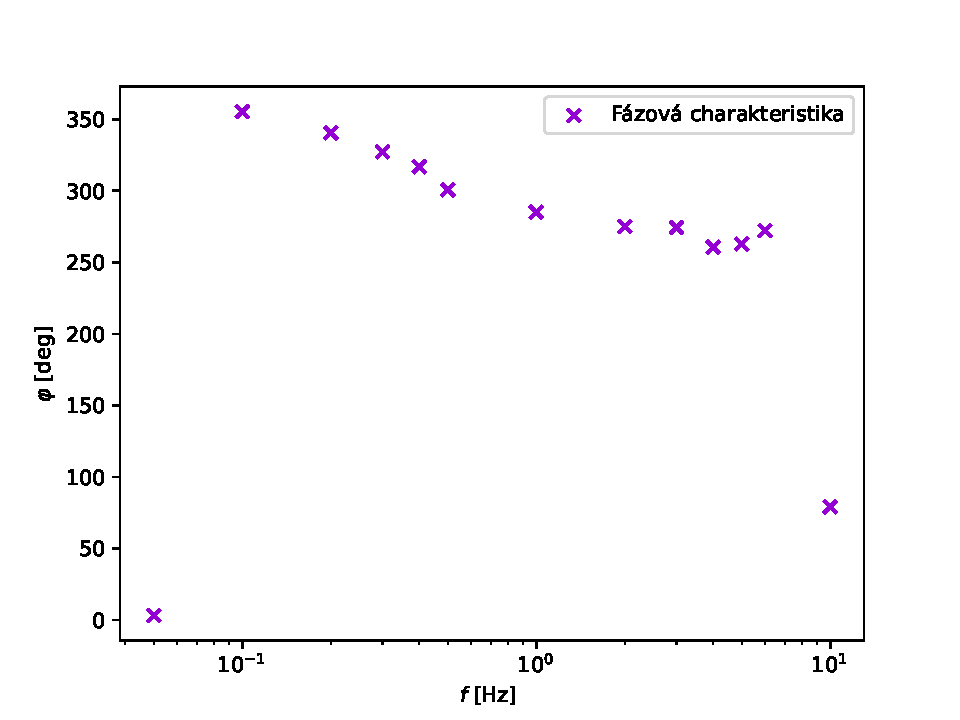
\includegraphics[]{img/graf_fazova_otevrena.pdf} %nejdůležitější řádek - obsahuje cestu k obrázku a také jeho relativní šířku k šířce textu
			%všiměte si, že je možné vložit obrázek vnořený ve složce img - tam poté můžete ukládat další obrázky 
			\caption{...} %popisek obrázku, který se zobrazí pod obrázkem
			\label{fig:fazova} %interní popis obrázku, který použijete k odkazování se
		\end{figure}

	\subsection{Přechodová charakteristika v uzavřené smyčce}

	\subsection{Amplitudová a fázová frekvenční charakteristika v uzavřené smyčce}
		\begin{figure}[!hbt] %bez této hranaté závorky se obrázek umístí na vrchol stránky
			\centering
			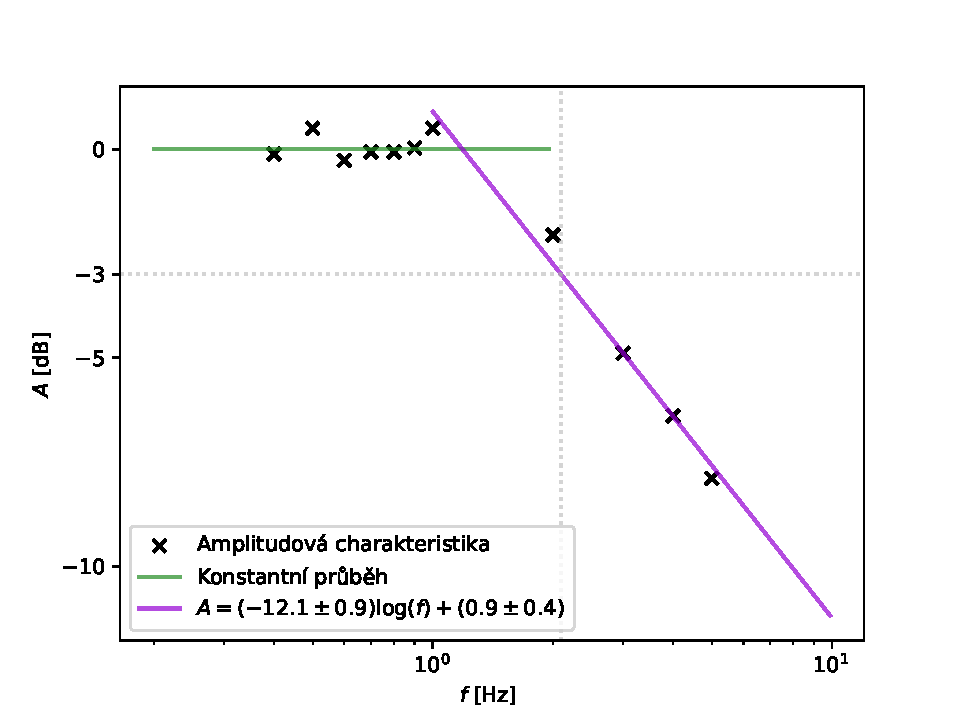
\includegraphics[]{img/graf_amplitudova_uzavrena.pdf} %nejdůležitější řádek - obsahuje cestu k obrázku a také jeho relativní šířku k šířce textu
			%všiměte si, že je možné vložit obrázek vnořený ve složce img - tam poté můžete ukládat další obrázky 
			\caption{$A=(-12.1\pm 0.9)log_10(f)+(-8.1\pm 0.4)$} %popisek obrázku, který se zobrazí pod obrázkem
			\label{fig:amplitudova_uzavrena} %interní popis obrázku, který použijete k odkazování se
		\end{figure}

		Prvním bodem vypracování by měl být odkaz na vypracovaný domácí úkol, který bývá většinou v části Příloha.
		Samotné vypracování všech pracovních úkolů, sekce by měla obsahovat všechny naměřené hodnoty (v případě extrémně velkých tabulek je možné je dát do přílohy) a grafy.
			Naměřené hodnoty se nachází v Tab.~\ref{tab:vzor}. Kód na psaní jednotek v hlavičce tabulky: \\ \verb|\tabh{I}{mA} & \tabh{v}{m \cdot s^{-1}}|.
				\begin{table}[!ht]
				  \centering
				    \begin{tabular}{|r|r|r|r|r|r|}
				    	\hline
				    	\tabh{I}{mA} & \tabh{v}{m \cdot s^{-1}} & \tabh{m}{kg}& \tabh{Q}{C} & \tabh{n}{mol} & \tabh{T}{\celsius} \\ \hline\hline
				    	     331 &                            -9 &      351 &       8 &     -0,53 &           0,64 \\ \hline
				    	     714 &                          -142 &      718 &     145 &     -0,07 &           0,07 \\ \hline
				    \end{tabular}
				  \caption{Popis vzorové tabulky. $I$ jsou naměřené hodnoty proudu, měřené s chybou $\pm1$ mA,\dots }
				  \label{tab:vzor}
				\end{table}
								
				
			
% ----------------------------------------------------------------------
%  Diskuse - obsahuje komentář k jednotlivým výsledkům, porovnání s očekáváním/tabulkovými hodnotami, zdroje především systematických chyb měření, návrh na zlepšení výsledků,...
% ----------------------------------------------------------------------			
	\section{Diskuse}			

% ----------------------------------------------------------------------
%  Závěr - stručně a jasně shrnout splněné cíle měření, úkoly a výsledky měření
% ----------------------------------------------------------------------
			
\section{Závěr}
	


